\style{mb} %pour microbit


\section{Les fonctions avec \mb}


\subsection{Description}

\subsubsection{Objectif}
%   bloc de formule
%   sans titre et fond bleu cyan
\begin{formule}
L'activité proposée vise à aborder la notion de fonction de façon ludique à l'aide de 2 \mb : l'un servant
à afficher l'antécédent et l'image, l'autre à calculer.\\~

On distingue ainsi le couple antécédent-image de la fonction qui les relie. Le but initial étant de détermier cette relation, puis d'en inventer d'autres.\\~
En terme de programmation, la réalisation demandée aux élèves est minime.
\end{formule}


\subsubsection{Intérêt}

L'utilisation de plusieurs \mb pour aborder les fonctions ,outre le côté ludique, va permettre par un jeu d'aller-retour
de distinguer les notions d'antécédent, d'image et de fonction. Bien souvent, on aborde les fonctions 
en évoquant le concept d'une boîte noire. Ici la boîte noire sera plus qu'un concept, ce sera un \mb !\\~

Cela va aussi donner d'évoquer la fonction au sens informatique du terme. Cependant, il faut noter que le bloc "fonction" de 
l'interface makecode s'il peut prendre des arguments, ne permet pas (pour l'instant) à une fonction de renvoyer un nombre (ou autre chose).\\~

En résumé, cette activité va permettre de :


%liste d'arguments
\begin{description}
    \item [Favoriser] une démarche de recherche en laissant libre cours au élève pour déterminer la relation.
    \item [Distinguer] la notion d'antécédent, d'image et de fonction
    \item [Programmer] des fonctions numériques
\end{description}


\subsubsection{Matériel}
\begin{itemize}
%   matériel pour micro:bit
    \item 2 $\times$ \matosMb \emph{(le simulateur ne suffira pas !)}
%   site pour micro:bit
    \item 1 $\times$ accès internet : IDE programmation par bloc \url{http://makecode.microbit.org/}

\end{itemize}


\newpage

\subsubsection{Élément pour la mise en oeuvre}

\begin{methode}
    Découpage de l'activité

    \begin{enumerate}
        \item \textbf{Découverte} \\
            Dans cette première phase, on explique aux élèves comment choisir un nombre 
            (en appuyant sur A et B pour incrémenter/décrémenter) avec le premier \mb et 
            comment envoyer (en secouant) ce nombre au deuxième \mb.\\
            On explique que ce deuxième \mb va faire un calcul avec ce nombre et qu'en le secouant, il 
            va renvoyer le nombre obtenu après calcul.\\~

            On doit donc donner comme objectif aux élèves de déterminer le calcul qui est effectué par le \mb "boite noire".
            

        \item \textbf{Programmation}\\
            En guise de deuxième phase, on pourra proposer aux élèves de prorammer eux-même une fonction
            et de mettre au défi leur camarade de déterminer la fonction. Pour cela il faudra leur fournir 
            le code du \mb "boite noire" et leur indiquer quelle partie du programme ils doivent modifier.
    
    \end{enumerate}
\end{methode}


\begin{remarque}
    Attention, il faudra veiller à bien définir des groupes "radio" différents pour chaque paire de \mb.
    Sinon, il y a un réel risque d'échange de nombres entre les différents groupes ce qui risque de créer une certaine confusion !\\~

    Les codes à utiliser :
    \begin{itemize}
        \item Pour le \mb "boite noire" : \url{https://makecode.microbit.org/_P2TCYDe1UHHt}.\\~
        
        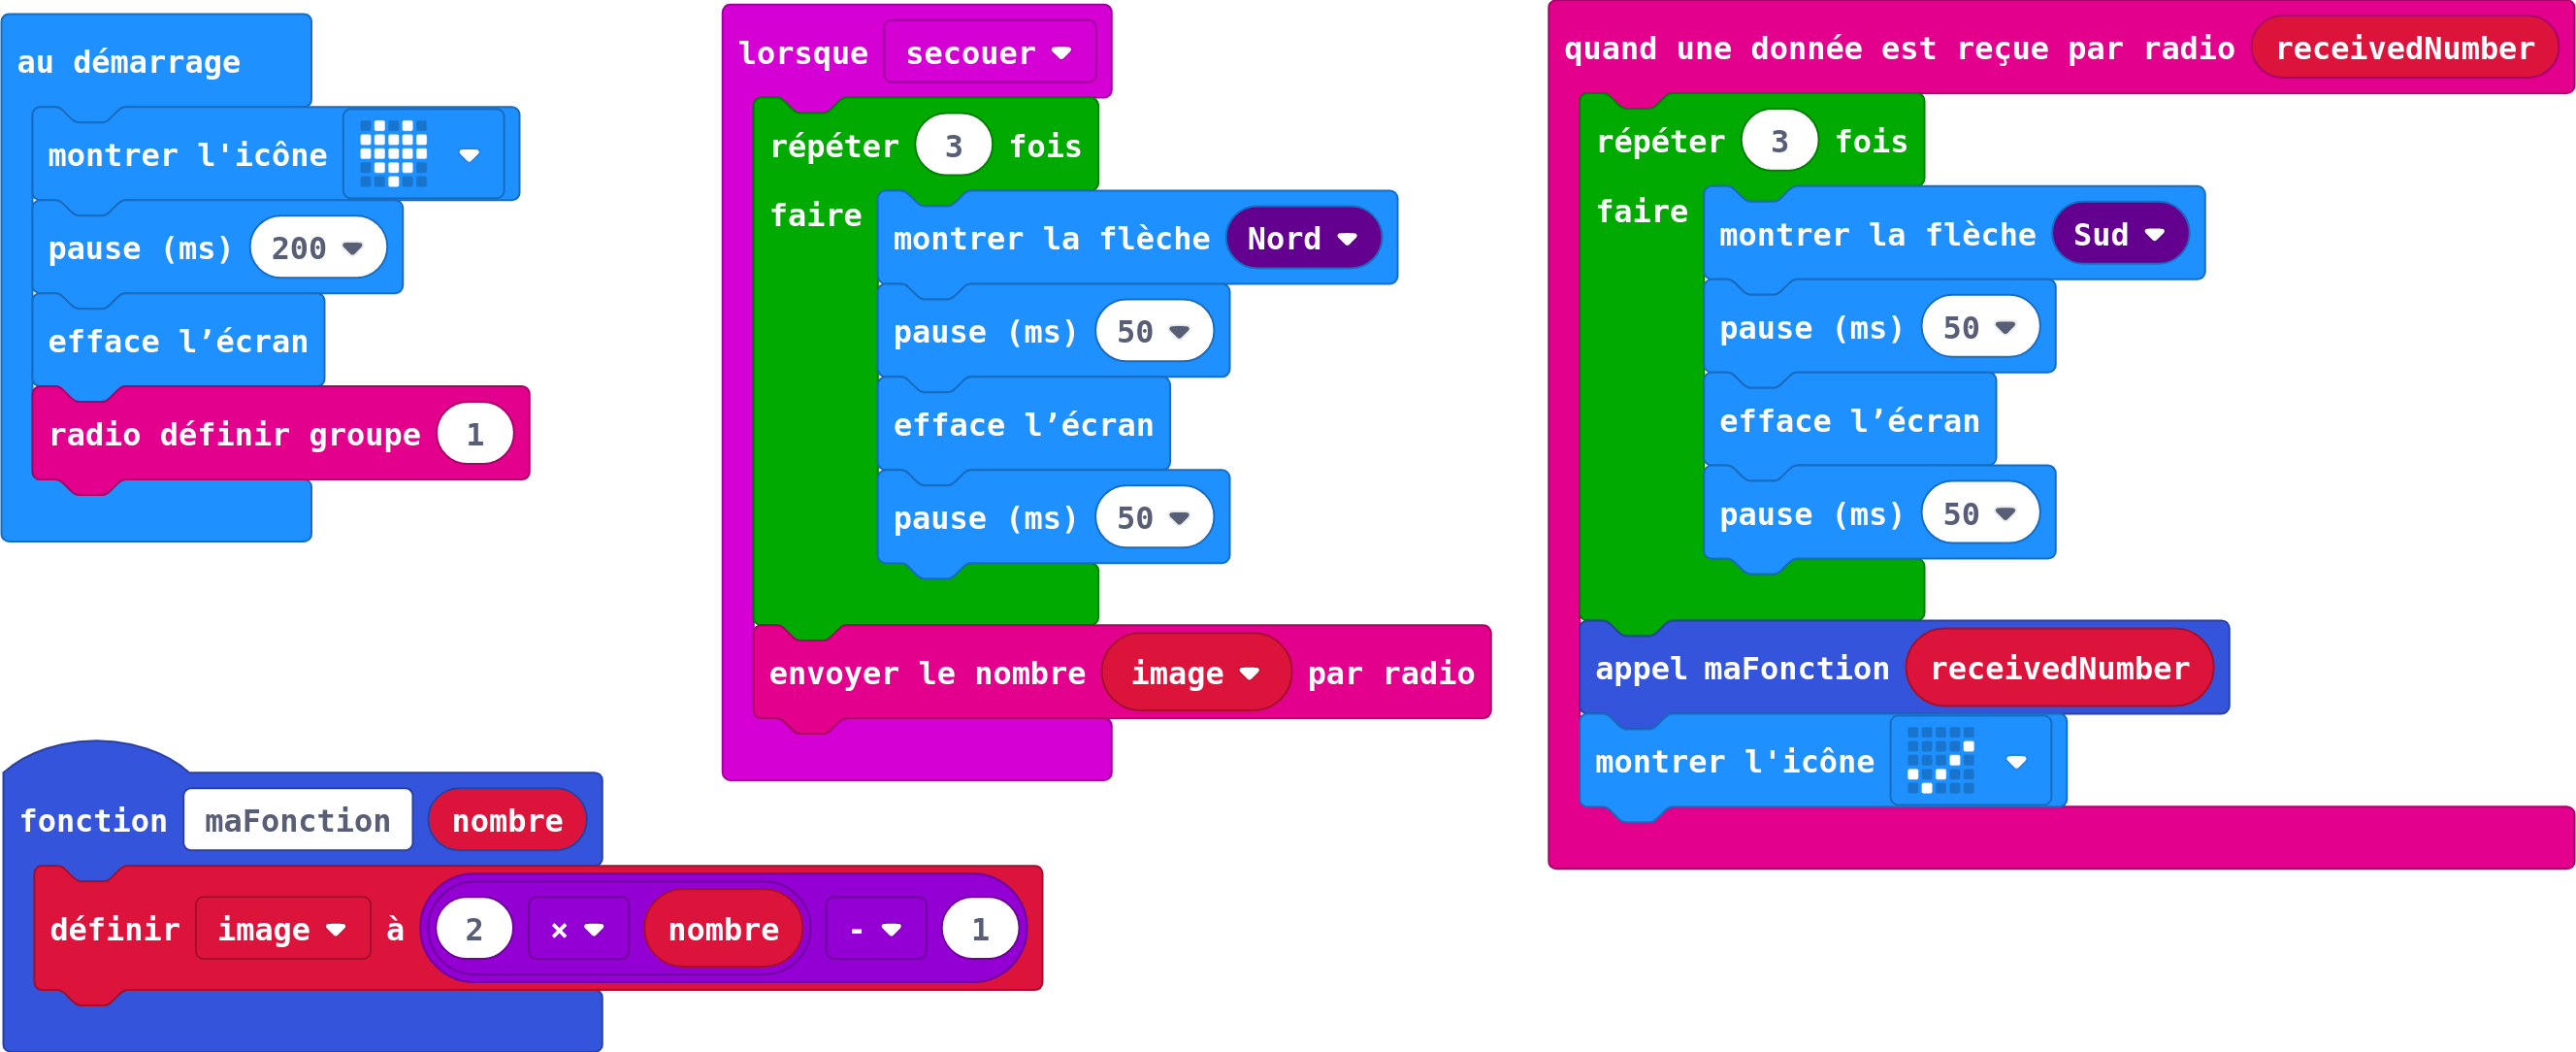
\includegraphics[width=0.8\linewidth]{res/mb-fonction-boite-noire.png}

        \item Pour le \mb "antécédent-image" : \url{https://makecode.microbit.org/_bC2LgWVYdEHp}.
        
        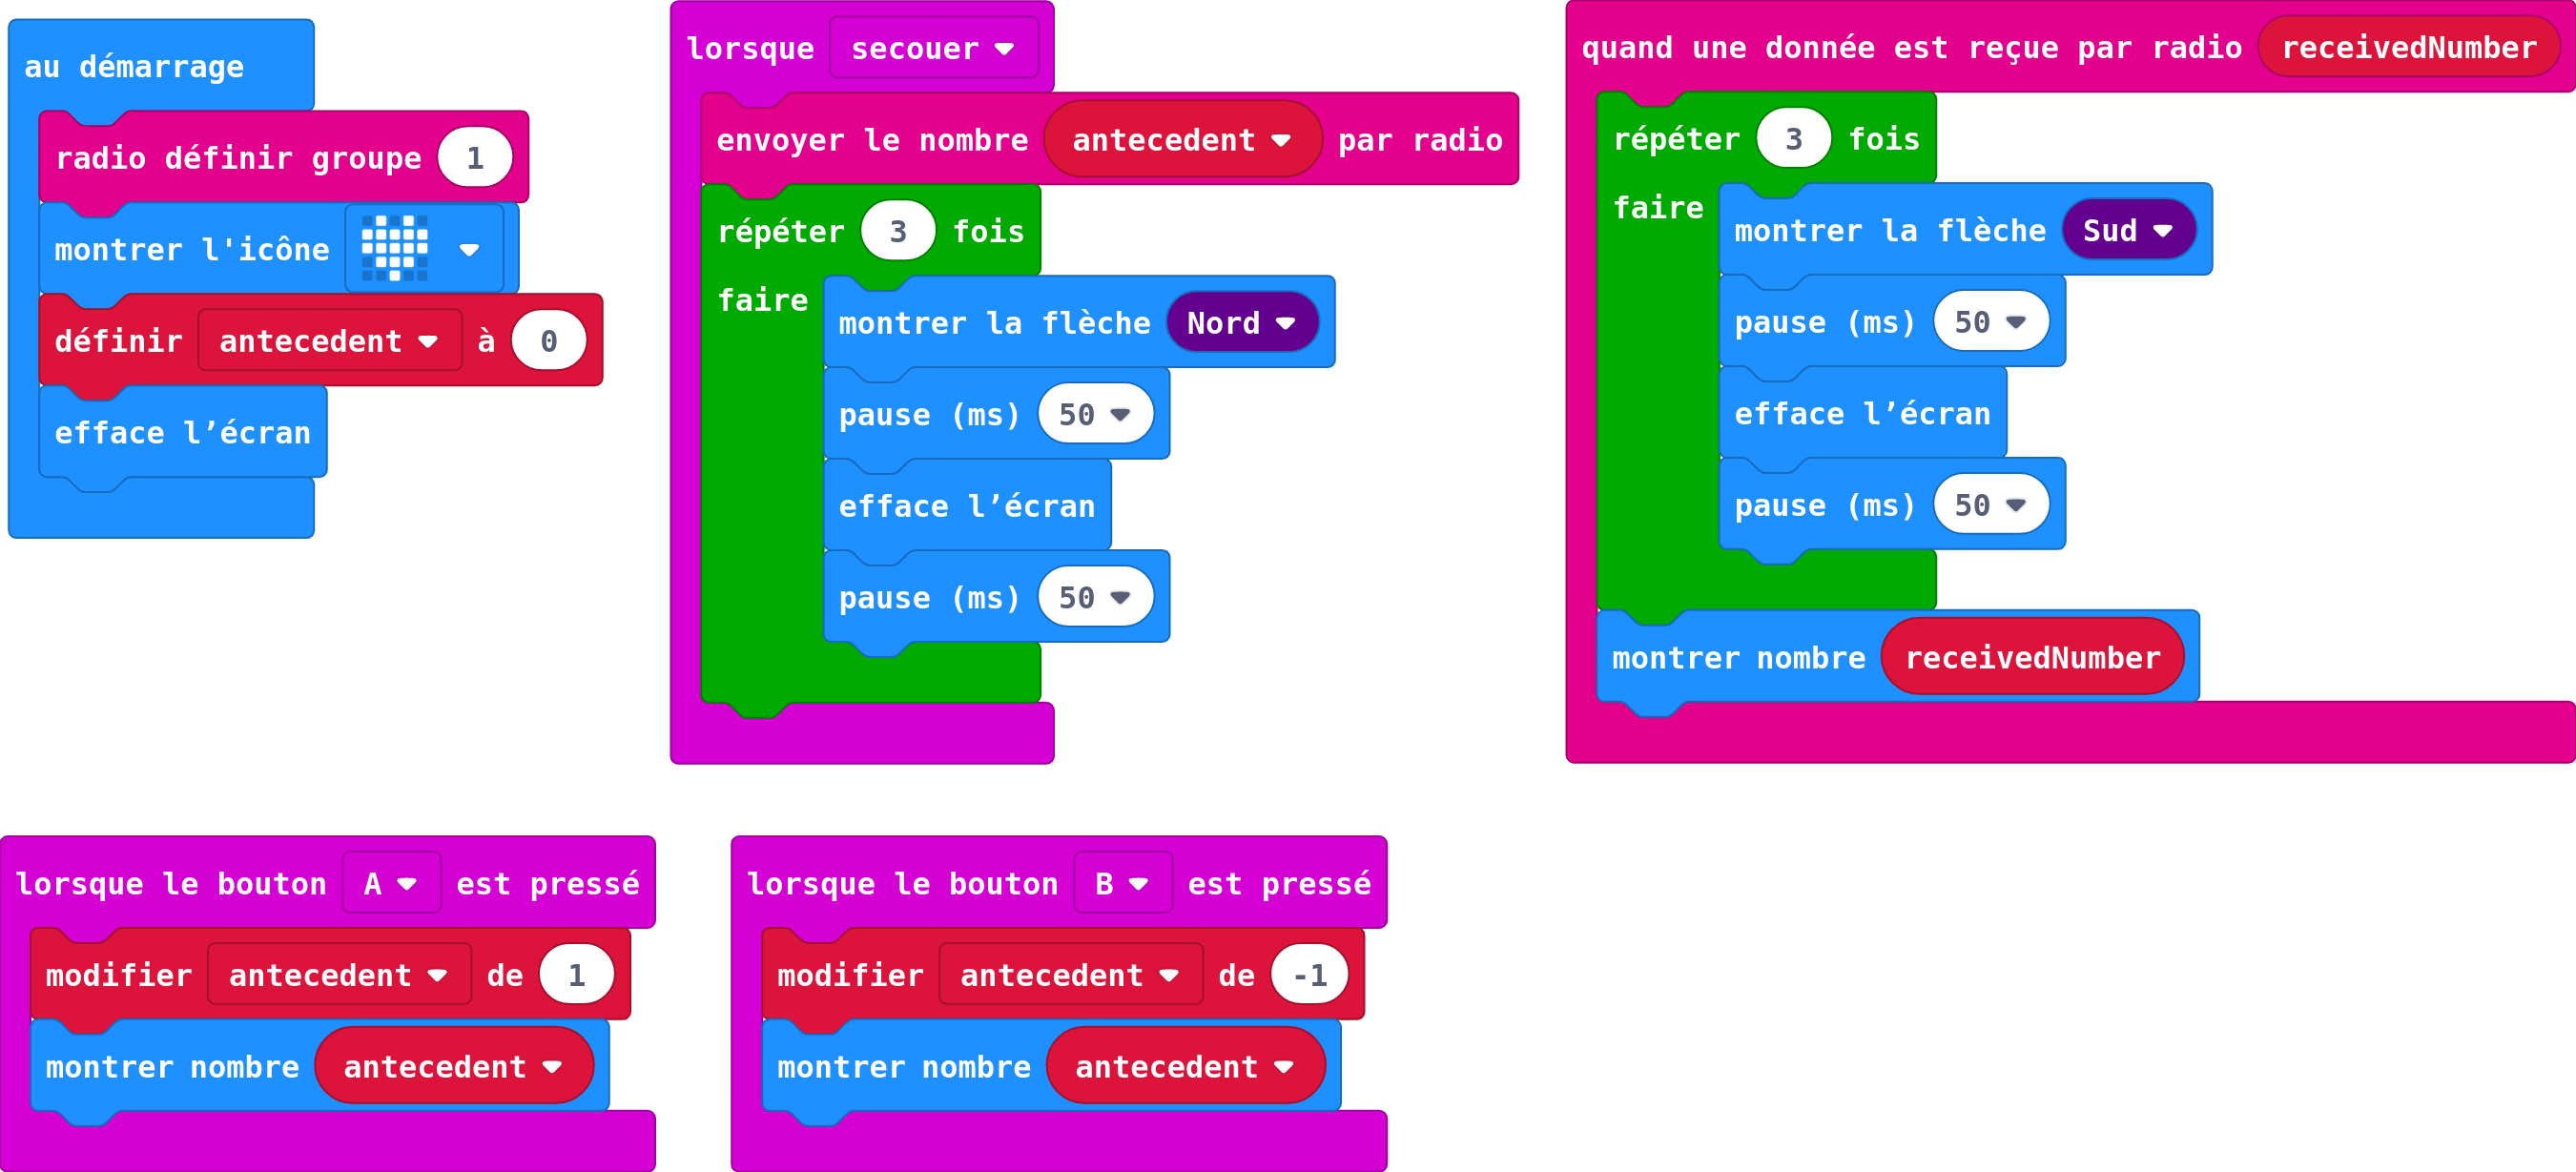
\includegraphics[width=0.8\linewidth]{res/mb-fonction-ant-img.png}
    \end{itemize}
   
\end{remarque}
